% ---------------------------------------------------------------------------------------------------------------
% This .tex source is an example which *does* use
% the .bib file (from which the .bbl file % is produced).
% REMEMBER HOWEVER: After having produced the .bbl file,
% and prior to final submission, you *NEED* to 'insert'
% your .bbl file into your source .tex file so as to provide
% ONE 'self-contained' source file.
%
% ===============================================================

\documentclass{sig-alternate-05-2015}

%\usepackage{qtree}
\usepackage{listings}
\usepackage[final]{pdfpages}
\usepackage{booktabs}
\usepackage{longtable}
\usepackage{graphicx}

% Drasil, short for Yggdrasil.

\newcommand{\lss}{Drasil}

\lstset{language=Haskell}

\begin{document}

% Copyright
\setcopyright{acmcopyright}
%\setcopyright{acmlicensed}
%\setcopyright{rightsretained}
%\setcopyright{usgov}
%\setcopyright{usgovmixed}
%\setcopyright{cagov}
%\setcopyright{cagovmixed}


% DOI
%\doi{10.475/123_4} %D What goes here?

% ISBN
%\isbn{123-4567-24-567/08/06}  %D What goes here?

%Conference
\conferenceinfo{SE4Science'16}{Austin, TX, USA}  %D What goes here?

% \acmPrice{\$15.00}  %D What goes here?

%
% --- Author Metadata here ---
% \conferenceinfo{SE4SC}{2016 ?, ? USA}  %D What goes here?
\CopyrightYear{2016} % Allows default copyright year (20XX) to be over-ridden - IF NEED BE.
%\crdata{0-12345-67-8/90/01}  % Allows default copyright data (0-89791-88-6/97/05) to be over-ridden - IF NEED BE.
% --- End of Author Metadata ---

\title{Position Paper: A Knowledge-Based Approach
to Scientific Software Development
%\titlenote{(Produces the permission block, and
%copyright information). For use with
%SIG-ALTERNATE.CLS. Supported by ACM.}}
%\subtitle{[Extended Abstract]
%\titlenote{A full version of this paper is available as
%\textit{Author's Guide to Preparing ACM SIG Proceedings Using
%\LaTeX$2_\epsilon$\ and BibTeX} at
%\texttt{www.acm.org/eaddress.htm}}
}

\numberofauthors{3} 
\author{
%D No idea what the ordering of this section should be
\alignauthor
Dan Szymczak\\
       \affaddr{McMaster University}\\
       \affaddr{1280 Main Street W}\\
       \affaddr{Hamilton, Ontario}\\
       \email{szymczdm@mcmaster.ca}
\alignauthor
Spencer Smith\\
       \affaddr{McMaster University}\\
       \affaddr{1280 Main Street W}\\
       \affaddr{Hamilton, Ontario}\\
       \email{smiths@mcmaster.ca} 
%D Not sure if you want your email machine-readable
\alignauthor
Jacques Carette\\
       \affaddr{McMaster University}\\
       \affaddr{1280 Main Street W}\\
       \affaddr{Hamilton, Ontario}\\
       \email{carette@mcmaster.ca}
}
\date{}

\maketitle
\begin{abstract}
As a relatively mature field, scientific computing has the opportunity to lead
other software fields by leveraging its solid, existing knowledge base.  By
following a rational design process, desirable software qualities such as
traceability, verifiability, and reproducibility, are arguable easier to reach
than for other classes of software.

We have begun development of a framework, \lss{}, to put this into practice.
Our aims are to ensure complete traceability, to facilitate agility in the
face of ever changing scientific computing projects, and ensure
that software artifacts can be easily and quickly extracted from \lss{}.
In particular, we are very interested in certifiable software and in
easy re-certification.

Using an example-based approach to our prototype implementation, we have
already seen many benefits. \lss{}
keeps all software artifacts (requirements, design, code, tests, build
scripts, documentation, etc) synchronized with each other. This allows for
reuse of common concepts across projects, and aids in the verification of
software. It is our hope that \lss{} will lead to the development of higher
quality software at lower cost over the long term.
\end{abstract}


%
%  Use this command to print the description
%
\printccsdesc

\keywords{Literate software, traceability, knowledge capture, software
  development, scientific computing, artifact generation.} %TODO

\section{Introduction}

We believe that, because of the solid scientific knowledge base built up
over the last $6+$ decades of work in Scientific Computing (SC), it is feasible
for SC to once again take a leadership position as regards the development
of high quality software.  More precisely, our goal is to use this knowledge
to improve the verifiability, reliability, usability, maintainability,
reusability and reproducibility of SC Software (SCS).

Some have argued for a rational document-drive design process 
\cite{SmithAndKoothoor2016}.  However, many researchers have
reported that a document driven process is not used by, nor suitable for, SCS;
they argue that scientific developers naturally use either an agile
philosophy~\cite{CarverEtAl2007, EasterbrookAndJohns2009, Segal2005}, or an
amethododical~\cite{Kelly2013} process, or a knowledge acquisition
driven~\cite{Kelly2015} process.  The arguments are that scientists do not
view rigid, process-heavy approaches, favourably~\cite{CarverEtAl2007} and that
in SC, requirements are impossible to determine up-front~\cite{CarverEtAl2007,
  SegalAndMorris2008}.  Rather than abandon the benefits of a rational
document-driven process, we argue that the appropriate tools can in fact
let the scientists focus even more of their time on science.

The principal perceived drawbacks of document-driven design methodologies are:
\begin{itemize}
\setlength{\itemsep}{0.0em}
\setlength{\parskip}{0pt}
\setlength{\parsep}{0pt}
\item information duplication,
\item synchronization headaches between artifacts,
\item an over-emphasis on non-executable artifacts.
\end{itemize}

Thus, to successfully achieve our goal of improving various software qualities
(verifiability, reliability, usability etc.) of SCS, whilst also improving,
or at least not diminish performance, we must also find a way to simultaneously
deal with the above drawbacks.  In fact, we are even more ambitious: we want
to improve developer productivity and thus save time and money on SCS
development, certification and re-certification. To accomplish this we need to
remove duplication between software artifacts \cite{WilsonEtAl2013} as well as
provide traceability between all software artifacts. In practice, this means
providing facilities for automatic software artifact generation from high level
``knowlege.'' We can accomplish this by have a single ``source'' for each
relevant piece of information which makes up an SC problem and its solution.
From this, we can generate all required documents and views.
That is, we aim to provide methods, tools and techniques to support a literate
process for developing scientific software that generalizes the idea behind
Knuth's~\cite{Knuth1984} literate programming.

%D May need to cut the roadmap for space.
In the following section, we  
%Section~\ref{sec:background} will give a more in-depth 
focus on SCS quality and literate programming.
%Section~\ref{sec:lss} 
Then we introduce our framework, \lss{}.  We show
a short example of the framework and discuss its advantages. 
%Section~\ref{sec:todo} will discuss
We then discuss how we want the framework to evolve. % and what future work we
%intend to do. %Finally, Section~\ref{sec:conclusion}  
The last section provides concluding remarks.

\section{Background} \label{sec:background}

In this section we discuss challenges for developing SCS and we
introduce the ideas behind our approach.

\subsection{Challenges} \label{ssec:challenges}

As the best numerical approach to solve a given problem is usually not known a
priori, we have to face the \textit{technique selection
  challenge}~\cite{Yu2011}. Experimentation is inevitably necessary to determine
the appropriate order of interpolation, the degree of implicitness,
etc. Nevertheless, the problem to solve does not change.  This implies that we
need a separation of concerns between the physical model and the numerical
algorithms.  Ease of experimentation means that we also need facilities to
parameterize algorithmic variabilities.

In an effort to make scientific libraries and software as widely applicable as
possible, most packages provide a generic interface with a large number of
options; this tends to overwhelm users and cause programmers to not reuse
libraries, since they do not believe the interface needs to be as complicated
as it appears~\cite{Dubois2002}. This is the \textit{understandability}
challenge~\cite{Yu2011}.  An ideal framework would expose an
API, as well as generate applications, which use routines which are only as
complicated as they need to be for the job at hand.

As requirements change, we face the \textit{maintainability
challenge}~\cite{Yu2011}.  The high frequency of change for SCS
causes accute problems for certification. If the expense and time required for
re-certification is on the same order of magnitude as the original
certification, changes will not be made. To be effective in this environment, a
framework needs to provide traceability, so the consequences of change can be
directly evaluated.

\subsection{Literate Programming} \label{ssec:literate}

Literate programming (LP) is a methodology introduced by Knuth
\cite{Knuth1984}. The main idea is to write programs in a way that explains 
{\bf (to humans)} what we want the computer to do, as opposed to simply giving
the computer instructions.

In a literate program, the documentation and code are together in one source.
While developing a literate program, the algorithms used are broken down into
small, understandable parts (known as ``sections'' \cite{Knuth1984} or
``chunks'' \cite{JohnsonAndJohnson1997}) which are explained, documented, and
implemented in an order which promotes understanding. To get working source
code, the \textit{tangle} process is run, which extracts the code from the
literate document and reorders it into an appropriate structure acceptable
to one's compiler.  Similarly, the \textit{weave} process is run to extract and
typeset the documentation.
There are several examples of SC programs being written in LP style, such as
VNODE-LP \cite{Nedialkov2006} and ``Physically Based Rendering: From Theory to
Implementation'' \cite{PharrAndHumphreys2004} (a literate program which is also
a successful textbook!).

\begin{figure}
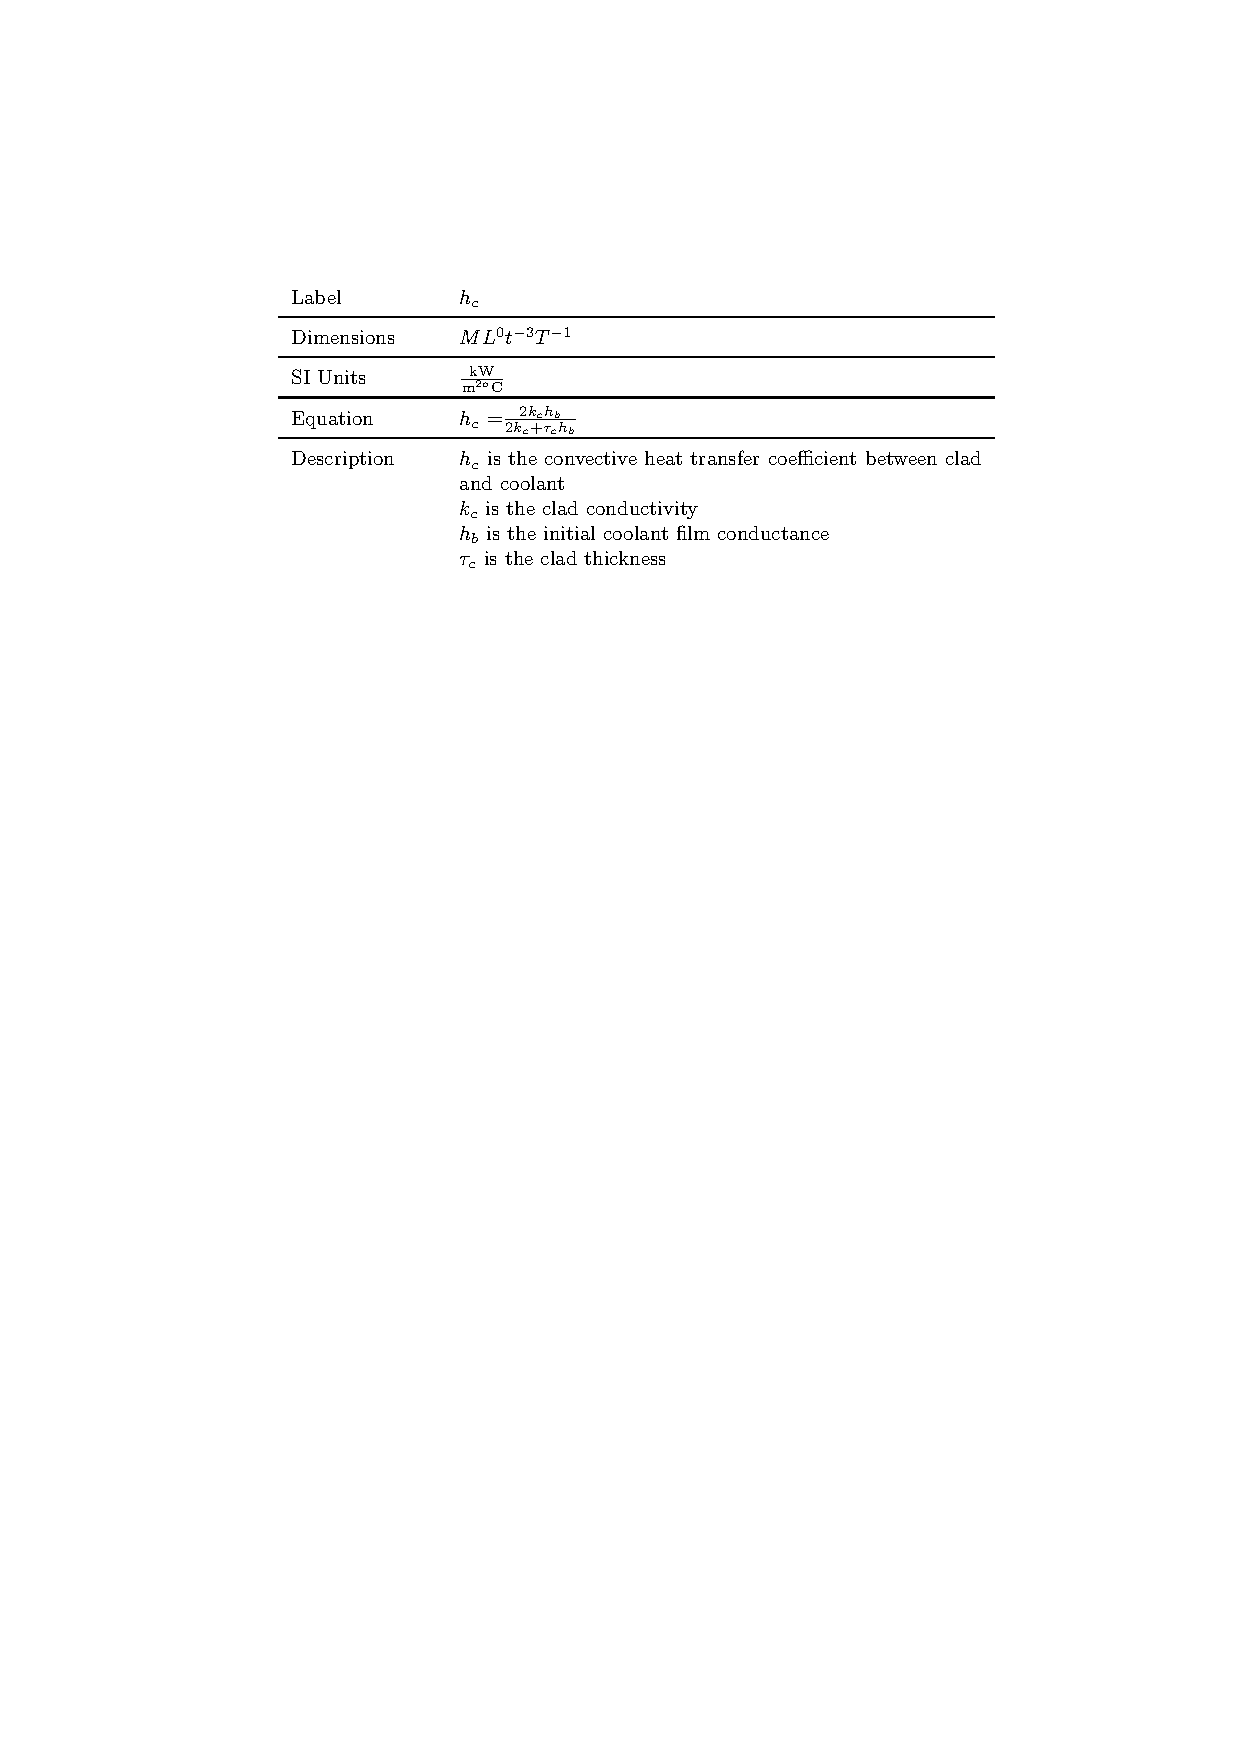
\includegraphics[width=0.49\textwidth]{h_c.pdf}
\caption{SRS data definition of $h_c$}
\label{fig:h_c}
\end{figure}	

\section{Introducing \lss} \label{sec:lss}

In \lss, we accomplish our two primary objectives (complete traceability, and
eliminating knowledge duplication) by generalizing the literate approach.

\subsection{A Simple Example} \label{ssec:example}

We have used a practical, example-driven approach to the development of \lss{}.
Our first example involves 
the simplified Software Requirements Specification (SRS) for a fuel pin in a
nuclear reactor (see \cite{SmithAndKoothoor2016} for more details). To get
started, let us look specifically at the term $h_c$ (defined in
Figure~\ref{fig:h_c}).  This defines a concept, its units, its
defining equation, and the description of the other concepts upon which it
depends.

We can currently generate the \verb|.tex| file for
much of the SRS for the fuel pin as well as the source code (in C) for the
required calculations.

\subsection{Design} \label{sssec:ex_how}

The fundamental task for \lss{} is \emph{knowledge capture}, in such a 
way that this knowledge can be viewed in different ways (code, specification,
etc).  Each individual piece of knowledge is a named \textit{chunk}; putting
chunks together is done via a \textit{recipe}; a \textit{generator} then
interprets recipes to produce the desired view.  

\begin{figure}
\begin{center}
{
 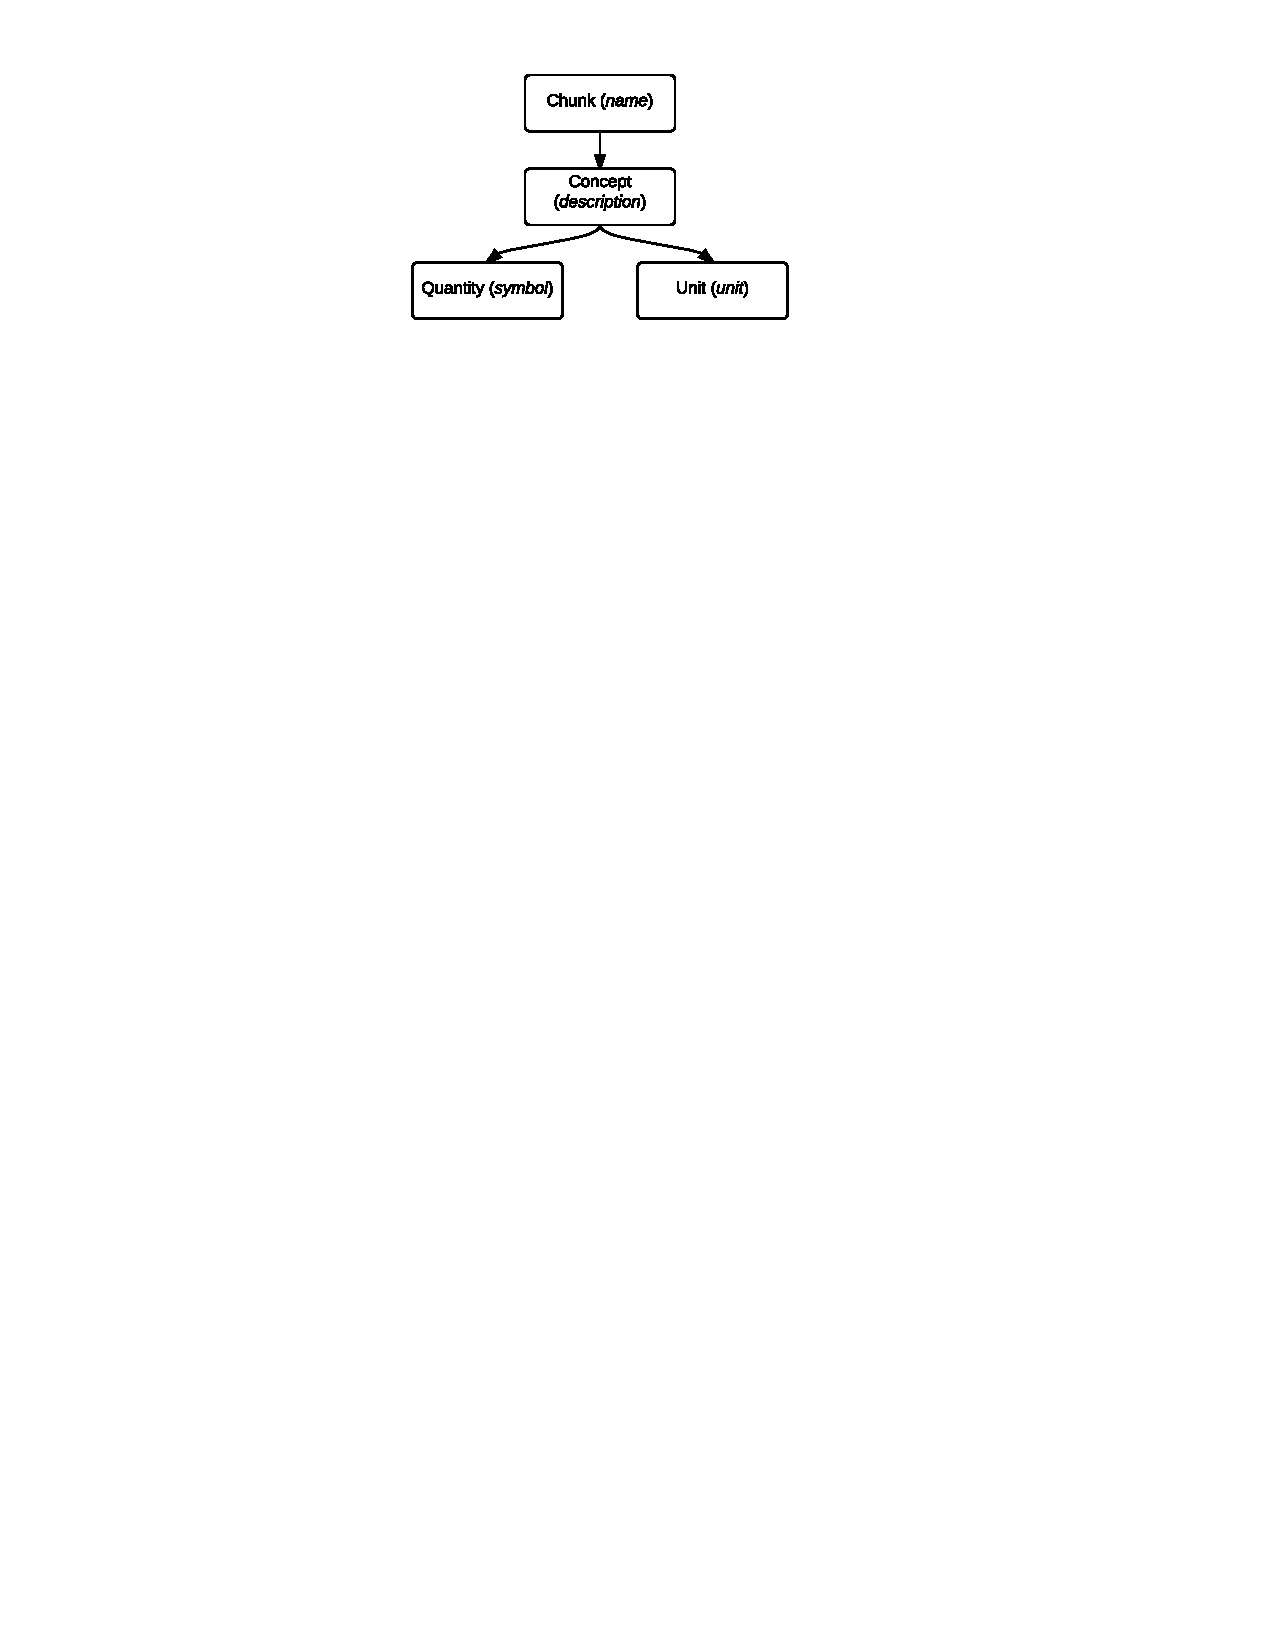
\includegraphics[width=0.35\textwidth]{ChunkHierarchy.pdf}
}
\end{center}
\caption{The chunk design}
\label{fig:chunks}
\end{figure}

We have different kinds of chunks.  The most basic ones are simply named pieces
of information.  Most however represent some \emph{concept}, which has a
\emph{description}.  In the SC context, many concepts are \emph{quantities},
which are represented by a specific \emph{symbol}.  Orthogonally, a \emph{unit}
is also a concept.  Most quantities have units.  And so on (as pictured
in Fig.~\ref{fig:chunks}).

By breaking things down in this way, we can assemble most concepts from
pre-existing chunks -- see Fig.~\ref{fig:recipe} for an SRS recipe that
uses $h_c$.

\begin{figure}[tb]
\begin{lstlisting}[frame=single, 
  showstringspaces=false, basicstyle=\scriptsize]
srsBody = srs [h_g, h_c] "Spencer Smith" [s1,s2]

s1 = Section (S "Table of Units") [intro, table]

table = Table 
 [S "Symbol", S "Description"] (mkTable
   [(\x -> Sy (x ^. unit)),
    (\x -> S (x ^. descr)) ] si_units)

intro = Paragraph (S "Throughout this ...")
\end{lstlisting}
\caption{A portion of the SRS recipe}
\label{fig:recipe}
\end{figure}

Currently, recipes are specified using a collection of DSLs embedded in
Haskell.  We have a DSL for expressions, expression layout, document
layout, C code, and LaTeX code.  For example, the expression layout DSL
describes how expressions should appear (subscript and
superscripts, concatenation of symbols, etc.), whereas the document layout
DSL deals with sections, tables, etc.

We have broken down our example into common knowledge, specific knowledge
and a recipe for an SRS (see Figure~\ref{fig:recipe}).
Here the fundamental SI units are common knowledge. Each is
contained within its own chunk in the SI unit library -- see
Figure~\ref{fig:know_common} for a taste.

\begin{figure}[thb]
\begin{lstlisting}[frame=single, showstringspaces=false, 
  basicstyle=\scriptsize]
metre, second, kelvin :: FundUnit
metre  = fund "Metre"  "length (metre)"       "m"
second = fund "Second" "time (second)"        "s"
kelvin = fund "Kelvin" "temperature (kelvin)" "K"
\end{lstlisting}
%mole   = fund "Mole"   "amount of substance (mole)"   "mol"
%kilogram = fund "Kilogram" "mass (kilogram)"      "kg"
%ampere   = fund "Ampere"   "electric current (ampere)"    "A"
%candela  = fund "Candela"  "luminous intensity (candela)" "cd"
\caption{Segment of the SI unit library}
\label{fig:know_common}
\end{figure}

The $h_c$ chunk (Figure~\ref{fig:know_specific}) is specific
knowledge: it contains the name, description, symbol, units, and equation
for $h_c$.

\begin{figure}
\begin{lstlisting}[frame=single, showstringspaces=false, basicstyle=\small]
h_c_eq :: Expr
h_c_eq = 2*(C k_c)*(C h_b) /
  (2*(C k_c) + (C tau_c)*(C h_b))

h_c :: EqChunk
h_c = fromEqn "h_c" 
 "convective heat transfer coefficient between 
    clad and coolant"
   (sub h c) heat_transfer h_c_eq
\end{lstlisting}
\caption{The $h_c$ chunk}
\label{fig:know_specific}
\end{figure}

The internal expression language \lstinline|Expr|
allows for the straighforward generation of source code. We utilize methods
similar to those found in \cite{SAGA:DSL, Szymczak2014}
wherein the expression language is converted to an abstract representation of
the code and then passed to a pretty-printer to create the final source.

We currently generate C code, however it would be possible to generate any
language provided we have an appropriate representation for that language.

\subsection{Advantages} \label{ssec:advantages}

We can already see some advantages over traditional SC
development. How \lss{} addresses the specific challenges of
Section~\ref{ssec:challenges} will be explored below.

\subsubsection{Knowledge Capture} \label{sssec:adv_knowledge}

In SCS there are many commonly shared theorems, formulae, algorithms and
data-structures across different applications. For example consider the general
form of the conservation of thermal energy equation, widely used in variety of
thermal analysis applications, with each solving a different problem, or
modeling a different system.

Our approach aims to build libraries of knowledge that can be reused anywhere.
Each library should contain common chunks relevant to a specific application
domain (ex. thermal analysis) and each project should aim to reuse as much as
possible during development.

From our example, a common source of reused knowledge is the Syst\'{e}me
International (SI) units (Figure~\ref{fig:know_common}). They are commonly
used throughout all of SC, so why should they be redefined for each
project? Once the knowledge has been captured, it can simply be reused.
With \lss{} this is possible with minimal effort, allowing developers and
scientists to spend their valuable time on more important things.

\subsubsection{Software Certification} \label{sssec:adv_cert}

High-quality documentation is required to certify software, but its creation
should not impede a scientists' work.  Major problems in creating SC software
stem from the maintainability and technique selection challenges
(Section~\ref{ssec:challenges}). As requirements and numerical algorithmic
decisions change, documentation and code must be updated.  This creates issues
with traceability and maintainability.

Depending on the regulatory body and the certification standards, many
types of documents may be required, such as requirements specification,
verification plans, design specification and code. \lss{} aims to generate these
documents alongside the code, while accounting for any changes. As the changes
will affect chunks and those chunks will be used to generate the documentation
and code, there is a guarantee that changes will propagate throughout all of the
artifacts.

In the context of re-certification, if a piece of software were developed using
\lss{} and some changes needed to be made, updating the artifacts and submitting
them for re-certification would be straightforward. All documentation would be
generated from the (newly modified) chunks, according to their existing recipes.
Or in the case of new information being added, a new chunk would be created and
the recipe slightly modified. During the implementation of our example, we have
already seen how \lss{} allows us to make changes at trivial cost.

On another note, if a document standard were to be changed during the
development cycle, it would not necessitate re-writing the entire document. All
of the information in the chunks would remain intact, only the recipe would need
to be changed to accommodate the new view. Thus, capturing all of the knowledge
that a program is based on and improving reproducibility.

%D This next section really feels like it's making a promise without really
%  explaining how/why it'll work.
\subsubsection{"Everything should be made as simple as possible, but not
  simpler."  (Einstein quote)} \label{sssec:adv_simple}

Currently there exist many powerful, general commercial programs for solving
problems using the finite element method. However, they are not often used to
develop new ``widgets'' because of the understandability challenge.
%cost and complexity of doing so~\cite{TODO}. %D Where is this from?
Engineers often have to resort to building and testing prototypes, instead of
performing simulations, due to a lack of tools that can assist with their exact
set of problems. %D Citation needed?

Our approach will change that by ideally making prototyping trivial through
generating source code suited to the needs of the engineers. Changes in
specifications could be seen in the code in (essentially) real-time at trivial
cost. For example, if an engineer were designing parts for strength, they could
have a general stress analysis program. This program could be 3D or specialized
for plane stress/strain, depending on which assumption would be most appropriate
at the time. The program could even be customized to the parameterized shape of
the part the engineer is interested in. The new program could only expose the
degrees of freedom necessary for the engineer to change (ex. material properties
or specific dimensions of the part), making the simulation process simpler and
safer.

\lss{} tackles this understandability challenge (Section~\ref{ssec:challenges})
by allowing developers to build components which will provide exactly what is
needed, no more and no less.

\subsubsection{Verification} \label{sssec:adv_verify}

When it comes to verification, requirements documents typically include
so-called ``sanity'' checks that can be reused throughout subsequent phases of
development. For instance, a requirement could assume conservation of mass or
constrain lengths to be always positive. The former would be used to test the
output and the latter to guard against invalid inputs.

With \lss, these sanity checks can be ensured by the knowledge capture
mechanism. Each chunk can maintain its own sanity checks and incorporate them
into the final system to ensure all inputs and outputs (including
intermediaries) are valid.

Also, with \lss{}, complete traceability is achievable through the use of
chunks, provided the requisite knowledge can be appropriately encapsulated.

Finally, any mistakes that occur in the generated software artifacts will occur
\textbf{everywhere}. Errors propagate through artifacts, and the artifacts will
always be in sync with each other (and the source). As a consequence, errors
will be much easier to find and only need to be fixed in one place.

\section{Future work} \label{sec:todo}

Currently the framework is still very small, producing only one document type
(the SRS) and only one type of code (C code for calculations). We plan to expand
\lss{} in several ways including, but not limited to:

\begin{enumerate}
\setlength{\itemsep}{0pt}
\setlength{\parskip}{0pt}
\setlength{\parsep}{0pt}
\item Generate more artifact types. %(i.e. have more default recipes).
\item Generate different document views. %(ex. SRS with equation derivations).
\item Include more types of information in chunks (see Table\ref{tab:pcm}).
\item Auto-generate test cases using constraints and typical values. The
  constraints should determine error cases, and typical value ranges give
  warnings.
\item Continue to expand the tool by implementing larger example systems.
\end{enumerate}

\begin{table} \label{tab:pcm}
\centering
\caption{Future knowledge to capture}
\begin{tabular}{|c|c|r|c|} \hline
\textbf{Var} & \textbf{Constraints} & \textbf{Typical Value} & \textbf{Uncertainty}\\ \hline
$L$ & $L > 0$ & 1.5 m & 10\% \\ \hline
$D$ & $D > 0$ & 0.412 m & 10\% \\ \hline
$V_P$ & $V_P > 0$ (*)	& 0.05 m$^3$	& 10\% \\ \hline
$A_P$ & $A_P > 0$ (*)	& 1.2 m$^2$	& 10\% \\ \hline
$\rho_P$ & $\rho_P > 0$	& 1007 kg/m$^3$	& 10\% \\
\hline\end{tabular}
\end{table}

For the auto-generation of test cases, physical constraints will be seen as hard
limits on values (ex. length must always be positive and a negative value would
throw an error). Typical values, on the other hand, are ``reasonable'' values
(ex. the length of a beam should be on the order of several metres, but
theoretically it could be kilometres, thus the code will raise a warning instead
of an error).

    
\section{Concluding Remarks} \label{sec:conclusion}

The current standard of using agile approaches to SC software development leave
many things to be desired. Documents tend to fall out of sync with the source
with each iteration, and the amount of hand-duplicated information leads to
errors affecting the quality of the software.

We have begun the creation of a framework to help ensure complete traceability
between software artifacts in the development process, while attempting to
inconvenience the developers as little as possible. Using our framework will
hopefully lead to higher quality software at very little cost.

\bibliographystyle{abbrv}
\bibliography{drasil}  
\end{document}
